%#! platex UserGuideJa
\chapter{\OFtool{FoamX}ケースマネージャ(v1.5では廃止)}
\label{chap:A}
\index{ケースマネージャ!FoamX@\OFtool{FoamX}(廃止)}%
\index{FoamX@\OFtool{FoamX}(廃止)!OpenFOAMケースマネージャ}%
OpenFOAMは,ケースの実行を管理するための
\OFtool{FoamX}ユーティリティと一緒に提供されています.
\OFtool{FoamX}はGUIであり,ほとんどの場合はローカルマシンの
ケースの管理に使われていますが,
インターネットのようなネットワーク上に割り当てられた
ケースを管理することもできます.

本章は主に,\OFtool{FoamX}に関する参考資料となっており,
\autoref{sec:A.3}と\autoref{sec:A.4}で
\OFtool{FoamX}の一般的な使い方に関する有効なアドバイスを提示していますが,
新規のユーザは\OFtool{FoamX}の使い方を習得するために,
最初にチュートリアル(\autoref{chap:2})を参照して下さい.

ネットワーク上でケースを実行するメカニズムは,
他のマシンのJAVA GUIから呼び出すことができるサービスを提供する
ホストマシンをもつことによって成立しています.
JAVA GUIとこれらサービス (ホストブラウザ,ケースブラウザ,
およびケースサーバ.C++で書かれています.) の間のインタフェースは,
\index{CORBA}%
Common ObjectRequest Broker Architecture (CORBA) を実装しているMICOです.
ローカルのマシンでケースを管理するだけの場合には,
そのマシンからホストブラウザとJAVA GUIの両方を立ち上げることができます.

以下のセクションにおいては,これをノーマルモードとすることにします.
オプション類を以下に要約します.
\begin{description}
 \item[ローカルでホストブラウザが実行(ノーマルモード)]
            この場合には,ユーザは
\index{runFoamX@\OFtool{runFoamX}!スクリプト/エイリアス|(}%
\index{スクリプト/エイリアス!runFoamX@\OFtool{runFoamX}|(}%
            \OFtool{runFoamX}を実行させることにより,
            ホストブラウザとGUIの両方を立ち上げることができます.
\begin{OFterminal}
\begin{verbatim}
runFoamX
\end{verbatim}
\end{OFterminal}
 \item[リモートでホストブラウザが実行(リモートモード)]
            この場合には,最初に
\index{runFoamXHB@\OFtool{runFoamXHB}!スクリプト/エイリアス}%
\index{スクリプト/エイリアス!runFoamXHB@\OFtool{runFoamXHB}}%
            \OFtool{runFoamXHB}によって,
            ホストブラウザがホストマシン上で立ち上げられます.
\begin{OFterminal}
\begin{verbatim}
runFoamXHB
\end{verbatim}
\end{OFterminal}
            そして実行中のホストブラウザに接続する\OFtool{runFoamX}を実行することにより,
            GUIがローカルで立ち上げられます.
\begin{OFterminal}
\begin{verbatim}
runFoamX
\end{verbatim}
\end{OFterminal}
\end{description}
これらのオプションの中に含まれているプロセスを\autoref{fig:A.1}に示します.
\OFtool{runFoamX}が実行されるとき,
\OFtool{runFoam}は実行中のホストブラウザを探します.
どれか一つが実行中であれば,
すなわち先に\OFtool{runFoamXHB}が立ち上がっていれば,
\OFtool{runFoamX}はこれに接続します.
そうでなければ,自分自身がホストブラウザを起動します.
\autoref{sec:A.1},\autoref{sec:A.2},\autoref{sec:A.3}では,
\OFtool{FoamX}の一般的な操作方法が,
ネットワーク上でどのように操作されるかを特に強調しながら述べられています.
続いて\autoref{sec:A.4}では,
ケースサーバを通じたOpenFOAMのケースの実行について述べられ,
\autoref{sec:A.5}では\OFtool{FoamX}に関係した設定について述べられています.


\begin{figure}[ht]
 
\includegraphics{fig-A-1}
 \caption{\OFtool{FoamX}実行のオプション}
 \label{fig:A.1}
\end{figure}



\section{ネームサーバとホストブラウザ}
\label{sec:A.1}
\index{FoamX@\OFtool{FoamX}(廃止)!ネームサーバ}%
\index{FoamX@\OFtool{FoamX}(廃止)!ホストブラウザ}%
\index{ネーム!サーバ}%
\index{ホスト!ブラウザ}%
ホストマシン上で\OFtool{FoamX}のホストブラウザを起動させるためには,
\index{runFoamXHB@\OFtool{runFoamXHB}!スクリプト/エイリアス}%
\index{スクリプト/エイリアス!runFoamXHB@\OFtool{runFoamXHB}}%
\OFtool{runFoamXHB}スクリプトを走らせるか,
あるいはホストブラウザがローカルで動いているケース(ノーマルモード)では,
\OFtool{runFoamX}を走らせることで\OFtool{runFoamX}自身が
\OFtool{runFoamXHB}を立ち上げます.
\OFtool{runFoamX}の二つの機能を\autoref{fig:A.2}に示します.


\begin{figure}[ht]
 \begin{minipage}{.49\textwidth}
  \centering
  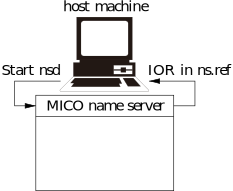
\includegraphics{fig-A-2-a}\par
  (a) ネームサーバ\OFtool{nsd}の起動
 \end{minipage}
 \begin{minipage}{.49\textwidth}
  \centering
  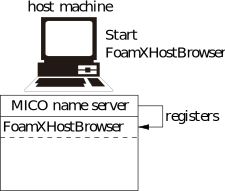
\includegraphics{fig-A-2-b}\par
  (b) \OFtool{FoamXHostBrowser}の起動
 \end{minipage}
 \caption{\OFtool{runFoamXHB}の実行}
 \label{fig:A.2}
\end{figure}


\begin{itemize}
 \item \OFtool{nsd}と呼ばれるプロセスであるMICOネームサーバは,
       ホストマシンからスタートされます.
       MICOはホストネームとデフォルトのポートアドレスを使用します.
       このポートアドレスは \OFpath{.OpenFOAM-1.5/apps/FoamX}ディレクトリの
       中にある
\index{FoamXClient.cfg@\OFpath{FoamXClient.cfg}!ファイル}%
\index{ファイル!FoamXClient.cfg@\OFpath{FoamXClient.cfg}}%
       \OFpath{FoamXClient.cfg}ファイルへの
       \texttt{org.omg.\allowbreak CORBA.ORBInitialHost}と
       \texttt{org.omg.CORBA.ORBInitialPort=} のエントリにより
       マニュアルで設定できます.
       ネームサーバは同じディレクトリの中にある\OFpath{ns.ref}に
       IORのhost/portを書き込みます.
 \item \OFkeyword{FoamXHostBrowser}プロセスは,
       \OFtool{nsd}がスタートされ,
       \OFkeyword{FoamXHostBrowser}という名で登録されている
       host/port上でスタートされます.
\end{itemize}
したがって,コマンドプロンプトで次のようにタイピングして
\OFtool{runFoamXHB}を実行することにより,
\begin{OFterminal}
\begin{verbatim}
runFoamXHB
\end{verbatim}
\end{OFterminal}
画面に以下のように出力させる
ネームサーバとホストブラウザが立ち上げられます.
\begin{OFterminal}
\begin{verbatim}
Starting NameServer with inet:<host>:<port>...
Starting FoamX Host Browser with inet:<host>:<port>...
\end{verbatim}
\end{OFterminal}
ここで,\verb|<host>:<port>| は,デフォルトで設定されているか,
あるいは\OFpath{FoamXClient.cfg}ファイルの中で指定されています.
\OFkeyword{FoamXHostBrowser}はOpenFOAMのロゴの商号と,
正しく実行しているかどうかのステータスの詳細を画面上に表示します.


\subsection{ネームサーバの実行に関する注記}
\label{ssec:A.1.1}
\OFpath{ns.ref}ファイルは,
以下のようにタイピングすることにより変換され,閲覧できます.
\begin{OFterminal}
\begin{verbatim}
iordump < $FOAMX_USER CONFIG/ns.ref
\end{verbatim}%$
\end{OFterminal}
MICOに関する管理者用ツールは,
以下のようにタイピングすることによりスタートします.
\begin{OFterminal}
\begin{verbatim}
nsadmin -ORBNamingAddr inet:<host>:<port>
\end{verbatim}
\end{OFterminal}
ここで,\verb|inet:<host>:<port>| エントリは,
\OFpath{ns.ref}ファイルを閲覧することにより見つけられます.
登録されたサービスをリストするために\texttt{ls}を含んでいる
ツールの中のオプションを閲覧するためには,\texttt{help}をタイプしてください.



\section{\OFemph{JAVA} GUI}
\label{sec:A.2}
\index{FoamX@\OFtool{FoamX}(廃止)!JAVA GUI@\OFemph{JAVA} GUI}%
すべてのリモートマシン,あるいはホストマシン自体は,
IORを提供するために先に作成され\OFpath{ns.ref}ファイルのコピーを使って,
ネームサーバに接続することができます.
リモートマシンでもまた,\OFpath{FoamXClient.cfg}ファイルの
ホストマシンの名前に設定するために,
\autoref{ssec:A.1.1}で述べた\OFpath{/etc/hosts}ファイルへの
対応する入力とともに,
\verb|org.omg.CORBA.ORBInitialHost=| を入力する必要があります.


\begin{figure}[ht]
 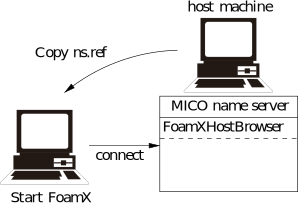
\includegraphics{fig-A-3-a}\par
 (a) ネームサーバへの接続\par
 \medskip
 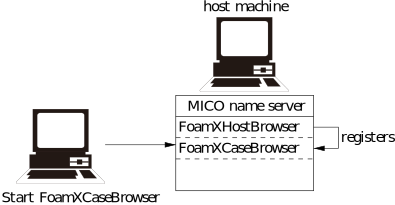
\includegraphics{fig-A-3-b}\par
 (b) FoamXCaseBrowserの実行
 \caption{\OFtool{runFoamX}の実行}
 \label{fig:A.3}
\end{figure}


\autoref{fig:A.3}~(a) に示しているように,
リモートマシンで\OFtool{FoamXJAVAGUI}をスタートするためには,
\index{runFoamX@\OFtool{runFoamX}!スクリプト/エイリアス|)}%
\index{スクリプト/エイリアス!runFoamX@\OFtool{runFoamX}|)}%
\OFtool{runFoamX}スクリプトを走らせる必要があります.
このスクリプトは\OFtool{runFoamXHB}により既に立ち上げられている
ネームサーバを探します.
ユーザは,このサーバに接続しようとすることを
認めるようコマンドラインで促されます.
\begin{OFterminal}
\begin{verbatim}
Found server reference \$FOAMX\_USER\_CONFIG/ns.ref
Do you want to connect to this server ? (n)
\end{verbatim}
\end{OFterminal}
ユーザが既存のネームサーバに接続しない場合や,
\OFtool{runFoamXHB}が実行されておらず,ネームサーバがない場合には,
新規のネームサーバがローカルに作成されます.
これにより,ホストブラウザとGUIの両方がローカルで走っているときは,
\OFtool{runFoamXHB}を走らせることなく,
\OFtool{runFoamX}を実行させれば十分です.
コマンドプロンプトで,次のようにタイピングすることにより,
\autoref{fig:A.4}に示すように,JAVAのブラウザ画面が開きます.
\begin{OFterminal}
\begin{verbatim}
runFoamX
\end{verbatim}
\end{OFterminal}
ブラウザは以下の領域に分割されています.
\begin{description}
 \item[Menu bar and buttons(上部)]
            ケースの作成と構築,および実行に用いる操作があります.
 \item[case panel(左側)]
            ケースブラウザの中のケースディレクトリと,
            ケースサーバの中のOpenFOAMのケースのコンテンツがあります.
 \item[Editing panel(右側ブルーの部分)]
            ケースの入力が修正されます.
 \item[Progress history panel(上部)]
            実行された動作に関する情報を提示するダイアログボックスです.
\end{description}


\begin{figure}[ht]
 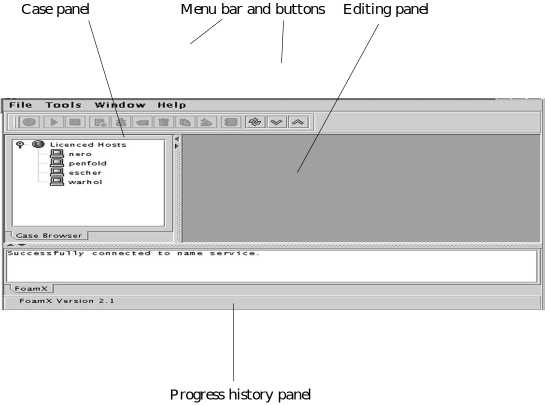
\includegraphics{fig-A-4}
 \caption{\OFtool{FoamX}のメイン・ブラウザ画面}
 \label{fig:A.4}
\end{figure}


デフォルトにより,ケースパネルはネームサーバが
走っているホストマシンを表示します.
他のリモートマシンのケースにアクセスしたい場合には
\OFpath{.OpenFOAM-1.5/controlDict}ファイルのホストに
マシンをリストする必要があります.
\OFtool{FoamX}の画面は,通常の方法で大きさの変更ができます.
\OFtool{FoamX}の中の個々の画面は,
画面を分割している斑点のバーをクリックし,
カーソルをドラッグすることにより大きさを変更できます.

ブラウザへのパスコマンドには3通りの方法があります.
\begin{itemize}
 \item アイテムを選択し,ダブルクリックします.
       一般的なコンテンツの開き方です.
 \item アイテムを選択し,マウスの右ボタンをクリックして,
       このアイテムで実行可能なメニューを表示させます.
 \item メニューバーとボタンからアイテムを選択することにより,
       他の操作を行うことができます.
\end{itemize}
注記:メニューボタンの上にカーソルを重ねると,
カーソルの下に小さいダイアログボックスが表れ,
簡単な用途の記述が表示されます.



\section{ケースブラウザ}
\label{sec:A.3}
\index{ケース!ブラウザ}%
\index{FoamX@\OFtool{FoamX}(廃止)!ケースブラウザ}%
JAVA GUIから,ケースパネルの中にリストアップされているマシンの
ケースブラウザを開くためには,ホストアイコンをダブルクリックするか,
あるいはシングルクリックでホストをハイライトさせて
メニューボタンかマウスの右のボタンから
Open Case Browserで選択します.
この操作は\autoref{fig:A.3}~(b) に示しているように,
\OFtool{FoamXCaseBrowser}を開くために
\OFtool{FoamXHostBrowser}を呼び出しています.
この\OFtool{FoamXCaseBrowser}はネームサーバを参照して
自らを登録するために\OFpath{ns.ref}ファイルを読み込みます.
その後,JAVA GUIは\OFtool{FoamXCaseBrowser}を
調べることができるようになり,
たとえばケース上で作業を開始するために
\OFtool{FoamXCaseServer}を起動するときに
\OFtool{FoamXCaseBrowser}を呼び出します.
\OFtool{FoamXCaseServer}は自らをネームサーバ上に登録し,
サービスを登録したり呼び出したりしてプロセスは続いていきます.

ケースブラウザは,引数としてホスト名をもたせて
\OFtool{runFoamX}を実行することにより,
JAVA GUIが立ち上がるときに自動的に開きます.
\begin{OFterminal}
\begin{verbatim}
runFoamX [host]
\end{verbatim}
\end{OFterminal}
ホストマシンでケースブラウザをスタートすると,
\autoref{fig:A.5}に示すように,
OpenFOAMが格納されているルートパスディレクトリの
ツリーのリストが作られます.
ユーザの \OFpath{.OpenFOAM-1.5/controlDict}ファイルの中で
指定されたケースのルートについて,
その追加や削除に関しては\autoref{ssec:A.5.2}を参照してください.


\begin{figure}[ht]
 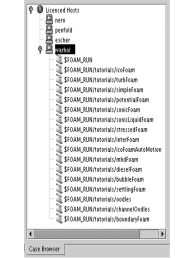
\includegraphics{fig-A-5}
 \caption{ケースのルートディレクトリのツリー}
 \label{fig:A.5}
\end{figure}


以下のマニュアルでの注意.
本文中に書かれた\OFtool{FoamX}に関するあらゆる操作は,
特に注記がない限り,メニューバーまたはボタンから,
あるいはマウスで右クリックすることにより選択されたものです.

\autoref{fig:A.6}に示すように,
ケースブラウザは一連の機能を提供しています.
ルートディレクトリのアイコンを選択することにより,
ユーザはディレクトリを開いたり,新しいケースを作成したり,
ケースをインポートしたり,ユーティリティを走らせることができます.
ケースの名前のアイコンをハイライトさせることにより,
ケースのオープン,削除,複製あるいは開放,
ケース上でのOpemFOAMのユーティリティの実行を行うことができます.


\begin{figure}[ht]
 \begin{minipage}{.49\textwidth}
  \centering
  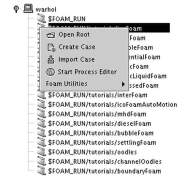
\includegraphics{fig-A-6-a}\par
  (a) ケース・ディレクトリの選択
 \end{minipage}
 \begin{minipage}{.49\textwidth}
  \centering
  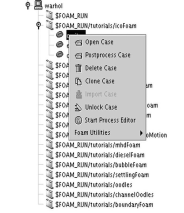
\includegraphics{fig-A-6-b}\par
  (b) ケース・ネームの選択
 \end{minipage}
 \caption{ケース・ブラウザの機能}
 \label{fig:A.6}
\end{figure}


\subsection{ルートディレクトリのオープン}
\label{ssec:A.3.1}
\autoref{fig:A.6}~(a) に示すように,
カーソルをルートディレクトリの上に置いて右クリックして
メニューを表示するか,
あるいはルートディレクトリのアイコンをダブルクリックすることで
Open Rootの機能を選択することにより,
ケースのルートディレクトリの中にある現在のケースのセットを
閲覧することができます.
\autoref{fig:A.7}に示すように,
ルートディレクトリのケースのツリーを表示するためにディレクトリを開きます.


\begin{figure}[ht]
 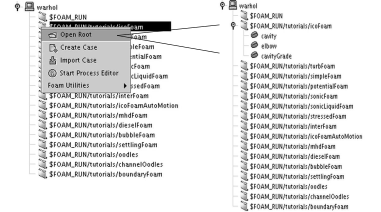
\includegraphics{fig-A-7}
 \caption{ケース・ルートを開く}
 \label{fig:A.7}
\end{figure}


\subsection{新規のケースの作成}
\label{ssec:A.3.2}
\autoref{fig:A.8}に示すように,メニューボタンから,
もしくはカーソルをホストのアイコンかケースのディレクトリの上に置いて
右クリックしてCreate Case機能を選択することにより,
新規のケースを作成することができます.
\autoref{fig:A.8}に示すように,
\index{Class@\OFkeyword{Class}!メニュー}%
\index{メニュー!Class@\OFkeyword{Class}}%
\OFkeyword{Class},
\index{Case Name@\OFemph{Case Name}!テキストボックス}%
\index{テキストボックス!Case Name@\OFemph{Case Name}}%
\OFemph{Case Name}および
\index{Case Root@\OFemph{Case Root}!テキストボックス}%
\index{テキストボックス!Case Root@\OFemph{Case Root}}%
\OFemph{Case Root}へのデータの登録ボックスを伴った小さなウィンドウが現れます.


\begin{figure}[ht]
 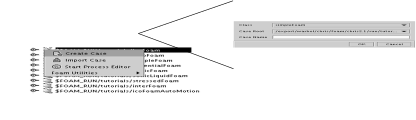
\includegraphics{fig-A-8}
 \caption{新規ケースの作成}
 \label{fig:A.8}
\end{figure}


Classは,\OFtool{icoFoam}や\OFtool{turbFoam}のような
OpenFOAMのソルバの名前を含んだスクロールメニューを提供しています.
\OFtool{FoamX}は,選択されたソルバにより要求されるケースファイルの中に
必要なデータを入力します.
したがって,正しいソルバを選ぶことは非常に重要です.
Case NameとCase Rootはそれぞれ,
ディレクトリパスとディレクトリ名となっており,
その中でケースのデータは,\autoref{sec:4.1}で述べてられている
ファイル構造にしたがって格納されています.
正しく入力できたらOKをクリックします.
新規のケースのケースサーバが開かれ,
\autoref{sec:A.4}で述べるように,ケースファイルの修正,
ソルバやユーティリティの実行などができるようになります.


\subsection{既存のケースを開く}
\label{ssec:A.3.3}
\autoref{fig:A.9}に示すように,Open Caseの機能は,
ケースサーバの中にある既存のケースを開きます.
\autoref{sec:A.4}で述べるように,ケースサーバではケースファイルの修正,
ソルバやユーティリティの実行ができるようになっています.


\begin{figure}[ht]
 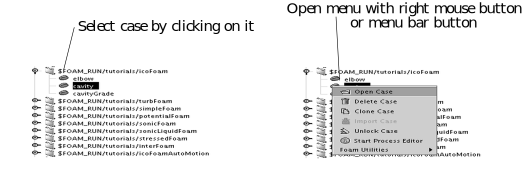
\includegraphics{fig-A-9}
 \caption{既存ケースを開く}
 \label{fig:A.9}
\end{figure}


\subsection{既存のケースの削除}
\label{ssec:A.3.4}
ハードディスクからケースディレクトリを削除するためには,
ケースをハイライトさせ,Delete Case機能を選択します.
\autoref{fig:A.10}に示すように,機能に関する画面が表示され,
削除するかどうかを聞いてきますので,
同意する場合にはYesボタンを,
そうでない場合にはNoボタンをクリックします.


\begin{figure}[ht]
 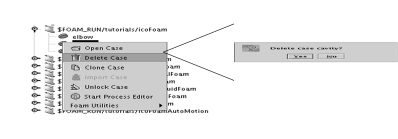
\includegraphics{fig-A-10}
 \caption{既存ケースの削除}
 \label{fig:A.10}
\end{figure}


\subsection{既存のケースの複製}
\label{ssec:A.3.5}
Clone Case機能は選択されたケースから既存のファイルをコピーする
新しいケースを作成します.
\autoref{fig:A.11}に示すように,
最初に複製をしたいケースをハイライトさせ,
Clone Case機能を選択する必要があります.
これによりテーブルを開きますが,
このテーブルの中で新しいケース名が指定されていなければならず,
またルートパスとapplicationClassは複製されるケースのものに
変更されるかもしれません.
最後に,\OFkeyword{times}の入力を行うことで複製の作業中にコピーされる
時刻ディレクトリを選ぶことができます.
このオプションを\autoref{tbl:A.1}に示します.


\begin{table}[ht]
 %#! platex UserGuideJa
\begin{tabular}{ll}
 オプション & 内容 \\
 \hline
\index{firstTime@\OFkeyword{firstTime}!メニューエントリ}%
\index{メニューエントリ!firstTime@\OFkeyword{firstTime}}%
 \OFkeyword{firstTime} & 最も古い時刻ディレクトリをコピーします \\
\index{latestTime@\OFkeyword{latestTime}!メニューエントリ}%
\index{メニューエントリ!latestTime@\OFkeyword{latestTime}}%
 \OFkeyword{latestTime} & 一番新しい時刻ディレクトリをコピーします \\
\index{allTime@\OFkeyword{allTime}!メニューエントリ}%
\index{メニューエントリ!allTime@\OFkeyword{allTime}}%
 \OFkeyword{allTime} & すべての時刻ディレクトリをコピーします \\
\index{noTime@\OFkeyword{noTime}!メニューエントリ}%
\index{メニューエントリ!noTime@\OFkeyword{noTime}}%
 \OFkeyword{noTime} & 時刻ディレクトリをコピーしません \\
 \hline
\end{tabular}

 \caption{Clone Case操作における時刻ディレクトリのコピーのオプション}
 \label{tbl:A.1}
\end{table}


的確な情報を入力し,Closeボタンをクリックすると,
複製操作が完了したことが知らされます.
\autoref{ssec:A.3.3}で説明しているように,
新しいケースを開くことができるようになります.


\begin{figure}[ht]
 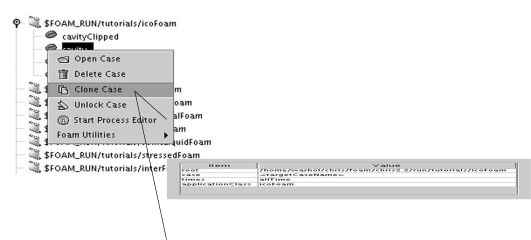
\includegraphics{fig-A-11}
 \caption{既存のケースの複製}
 \label{fig:A.11}
\end{figure}


\subsection{既存のケースを解放}
\label{ssec:A.3.6}
ケースが作成されているとき,あるいは開かれているときには,
このケースが異なるサーバでオープンされることを防ぐために
ロックファイルが作成されます.
ケースが閉じられるときには,再度開くことができるように,
このロックファイルは取り除かれます.
ある種の環境では,たとえケースサーバで
ケースがそれ以上進行できなくなるとしても,
ロックファイルは削除されないかもしれません.
例えば,ケースサーバでケースが開かれているのに
ホストブラウザが閉じられてしまうような場合がこれに該当します.
このため,Unlock Case機能は
ロックファイルを削除するオプションを備えています.
\autoref{fig:A.12}に示すように,
ケースが他のユーザによって進められているかもしれないことを
警告する画面が表示されます.
そのときには,ロックファイルの削除を受け入れる前に
他の場所でケースが進められていないことを
確認することはユーザの責任となります.


\begin{figure}[ht]
 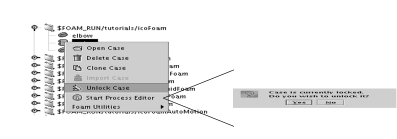
\includegraphics{fig-A-12}
 \caption{既存のケースのロックを解除する}
 \label{fig:A.12}
\end{figure}


\subsection{プロセスエディタ}
\label{ssec:A.3.7}
Start Process Editor機能は,
終了した,あるいは現在実行中のすべてのOpenFOAMのジョブを
モニタできるエディタを開きます.
エディタは単純なGUIで,インストール時に
\OFpath{\$FOAM\_LIC\_DIR}ディレクトリの中に置かれており,
\OFpath{runningJobs}と\OFpath{finishedJobs}のディレクトリにある
ファイルを読み込みます.
これは\autoref{fig:A.13}に示すような構成になっています.


\begin{figure}[ht]
 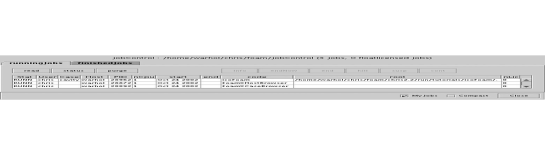
\includegraphics{fig-A-13-a}\par
 (a) 実行中のジョブ一覧\par
 \medskip
 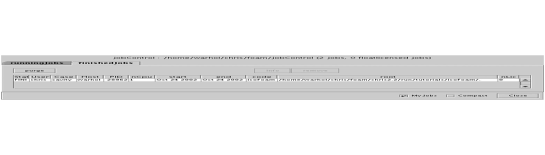
\includegraphics{fig-A-13-b}\par
 (b) 終了したジョブ一覧
 \caption{プロセスの管理}
 \label{fig:A.13}
\end{figure}


それは\autoref{fig:A.13}に示すような画面からなります.
タグで,\OFkeyword{runningJobs}テーブルと
\OFkeyword{finishedJobs}テーブルを切り替えられます.
テーブルは非常にわかりやすいジョブの詳細が入っています.
runningJobsテーブルの左上に\autoref{tbl:A.2}にリストアップされた
タスクを実行するボタンがあります.
runningJobsテーブル上でクリックすることによって,
ジョブを選択することもできます.
するとテーブルの右上のボタンが有効になります.
これらのボタンで,\autoref{tbl:A.2}に記載されているジョブを制御することができます.


\begin{table}[ht]
 %#! platex UserGuideJa
\begin{tabular}{ll}
 \multicolumn{2}{l}{メインボタン} \\
 \hline
\index{read@\OFemph{read}!ボタン}%
\index{ボタン!read@\OFemph{read}}%
 \OFemph{read} & runningJobsとfinishedJobsディレクトリのジョブを再度読込む \\
\index{status@\OFemph{status}!ボタン}%
\index{ボタン!status@\OFemph{status}}%
 \OFemph{status} & ジョブのステータスを更新するためにホストマシンに接続する \\
\index{purge@\OFemph{purge}!ボタン}%
\index{ボタン!purge@\OFemph{purge}}%
 \OFemph{purge} & これ以上実行しないジョブを取り除く \\
 \\
 \multicolumn{2}{l}{ジョブ実行ボタン} \\
 \hline
\index{Info@\OFemph{Info}!ボタン}%
\index{ボタン!Info@\OFemph{Info}}%
 \OFemph{Info} & ジョブの情報画面を表示する \\
\index{endNow@\OFemph{endNow}!ボタン}%
\index{ボタン!endNow@\OFemph{endNow}}%
 \OFemph{endNow} & 次のタイムステップでジョブを終わらせる \\
\index{end@\OFemph{end}!ボタン}%
\index{ボタン!end@\OFemph{end}}%
 \OFemph{end} & ジョブがフィールドデータをファイルに出力する次のタイムステップでジョブを終わらせる \\
\index{kill@\OFemph{kill}!ボタン}%
\index{ボタン!kill@\OFemph{kill}}%
 \OFemph{kill} & 即座にジョブを終了 \\
\index{suspend@\OFemph{suspend}!ボタン}%
\index{ボタン!suspend@\OFemph{suspend}}%
 \OFemph{suspend} & 即座にジョブを一時停止 \\
\index{cont@\OFemph{cont}!ボタン}%
\index{ボタン!cont@\OFemph{cont}}%
 \OFemph{cont} & 一時停止したジョブを再実行 \\
 \\
 \multicolumn{2}{l}{チェックボックス} \\
 \hline
\index{My Jobs@\OFemph{My Jobs}!ボタン}%
\index{ボタン!My Jobs@\OFemph{My Jobs}}%
 \OFemph{My Jobs} & 現在のユーザのジョブのみ見る \\
\index{Compact@\OFemph{Compact}!ボタン}%
\index{ボタン!Compact@\OFemph{Compact}}%
 \OFemph{Compact} & リストから\OFtool{FoamX}関連のジョブを取り除く \\
 \hline
\end{tabular}

 \caption{プロセスエディタボタン}
 \label{tbl:A.2}
\end{table}


finishedJobsテーブルはOpenFOAMで実行されたが何らかの理由で
終了されたジョブの情報のアーカイブです.
役立つ入力は保存して,そうでないものは削除することが自由にできます.
テーブルには入力を削除するための2個のボタンがあります.
パージボタンは7日以上前に終了しているジョブを削除します.
リムーブボタンはテーブルから選択された入力を取り除きます.

プロセスエディタ画面の下部に,\autoref{tbl:A.2}に記載してあるように,
どのジョブがrunningJobsテーブルに入り,
どのジョブがfinishedJobsテーブルに入るかを
管理するチェックボックスが二つあります.


\subsection{OpenFOAMユーティリティの実行}
\label{ssec:A.3.8}
Foam Utilities機能では,OpenFOAMユーティリティを実行することができます.
この機能はケースサーバでも提供されており,
そこで使う方がより一般的です.それについては\autoref{sec:A.4}で説明します.



\section{ケースサーバ}
\label{sec:A.4}
\index{ケース!サーバ}%
\index{FoamX@\OFtool{FoamX}(廃止)!ケースサーバ}%
ケースブラウザからケースを開くと,ケースサーバが起動します.
\autoref{fig:5.14}に示すように,
ケース画面にディレクトリのツリーが表示されます.
ユーザはケース画面の底部にあるタグを用いて
新規のケースとケースブラウザのやりとりを行うことができます.
ディレクトリのツリーには,トップレベルの3種類の入力項目があります.
\begin{description}
 \item[Dictionaries] ケースのコントロールと物理特性を設定する
            ディクショナリをもっています.
 \item[Fields] フィールドの初期条件と境界条件を設定します.
 \item[Mesh] メッシュの読み込みとインポート,
            メッシュのパッチに関する境界条件を設定します.
\end{description}


\begin{figure}[ht]
 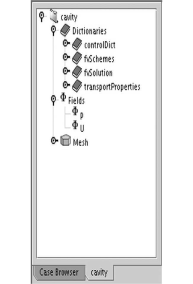
\includegraphics{fig-A-14}
 \caption{ケースサーバのウィンドウ}
 \label{fig:A.14}
\end{figure}


\subsection{既存のメッシュのインポート}
\label{ssec:A.4.1}
ケースにはメッシュが必要であり,
そのメッシュは\autoref{sec:5.3}で述べている
\OFtool{blockMesh}ユーティリティを使うか,
あるいはOpenFOAMのメッシュ変換機と結合した
サードパーティのソフトウエアを用いて作成されます.
OpenFOAMのメッシュはケースの\OFpath{constant/polyMesh}ディレクトリに
以下のものとして保存されます.
boundary,cells等のOpenFOAMのメッシュを構成するファイル.
OpenFOAMのメッシュを作成するために\OFtool{blockMesh}が使う
\OFdictionary{blockMeshDict}ファイル.あるいはその両方があります.
\autoref{fig:A.15}に示すように,ユーザはこれらすべてのファイルを
Import Meshファンクションを使って
既存の\OFpath{constant/polyMesh}ディレクトリから
それぞれのcaseにインポートします.


\begin{figure}[ht]
 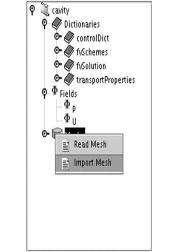
\includegraphics{fig-A-15}
 \caption{OpenFOAMのメッシュのインポート}
 \label{fig:A.15}
\end{figure}


\subsection{メッシュの読み込み}
\label{ssec:A.4.2}
\OFpath{constant/polyMesh}ディレクトリの中に,直接インポートされた,
または\OFtool{blockMesh}かメッシュの変換ユーティリティにより生成された
メッシュファイルが存在すると,Read Mesh\&Fields機能を用いて
ケースサーバにこれらを読み込むことができるようになります.


\begin{figure}[ht]
 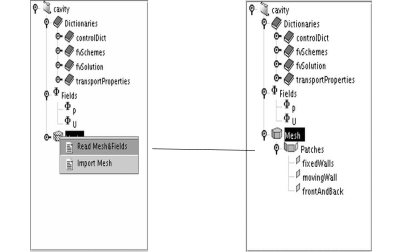
\includegraphics{fig-A-16}
 \caption{OpenFOAMメッシュの読み込み}
 \label{fig:A.16}
\end{figure}


この機能を試すには,チュートリアルの例のいずれかのファイルを開き,
\autoref{ssec:A.4.8}で述べている\OFtool{blockMesh}ユーティティを使って
メッシュを生成する必要があります.


\subsection{境界のパッチの設定}
\label{ssec:A.4.3}
\autoref{fig:A.16}に示すように,
Read Mesh\&Fields機能を実行した後は,
ディレクトリのツリーはメッシュに関する
境界のパッチのリストを表示するようになります.
その後,パッチをハイライトさせ,
Define Boundary Type機能を選択することにより,
物理的な境界条件をパッチに合わせることができます.


\begin{figure}[ht]
 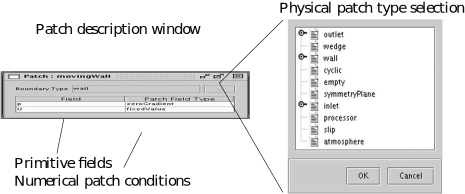
\includegraphics{fig-A-17}
 \caption{物理的境界条件の選択}
 \label{fig:A.17}
\end{figure}


これにより,編集パネルの中にpatch description(パッチの記述)画面が
表示されます.\autoref{fig:A.17}のイラストに示すように,
Boundary Typeの表示の右側の \ldots\ ボタンをクリックすることにより,
物理的な境界条件のタイプを選択することができます.
特定のソルバに利用可能な物理的な境界条件のタイプのリストが画面に現れます.
リストから選択して,OKをクリックすると,ウィンドウは閉じ,
patch description画面に戻ります.
物理的なBoundary Typeの表示の下には,
ソルバの初期変数や解析時のそれらのパッチタイプ,
または境界条件をリストした表があります.
このとき,2次元のケースにおいて一列に並んだ前後のパッチが
\index{きょうかいタイプ@境界タイプ!empty@\OFboundary{empty}}%
\index{empty@\OFboundary{empty}!きょうかいタイプ@境界タイプ}%
\OFboundary{empty}タイプになるように注意してすべてのパッチに対して
物理的な境界条件のタイプを選択します.


\subsection{フィールドの設定}
\label{ssec:A.4.4}
いったん全ての物理的なパッチタイプを決定すると,
いつものようにハイライトさせて右クリックするか
アイコンをダブルクリックすることによって選択される
\index{Fields@\OFemph{Fields}!ディクショナリツリー}%
\index{ディクショナリツリー!Fields@\OFemph{Fields}}%
\OFemph{Fields}は,
\OFkeyword{Edit Field}機能を使って編集できます.


\begin{figure}[ht]
 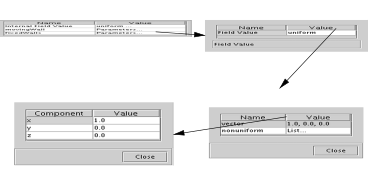
\includegraphics{fig-A-18}
 \caption{フィールドの編集とパッチ条件の設定}
 \label{fig:A.18}
\end{figure}


Edit Field機能は\autoref{fig:A.18}に示すように
編集パネルにフィールド画面を表示します.
表は\autoref{ssec:4.2.8}で概説した
各フィールドで必要な一連のデータ値を記載しており,
\index{internalField@\OFkeyword{internalField}!キーワード}%
\index{キーワード!internalField@\OFkeyword{internalField}}%
\OFkeyword{internalField}や
\index{referenceLevel@\OFkeyword{referenceLevel}!キーワード}%
\index{キーワード!referenceLevel@\OFkeyword{referenceLevel}}%
\OFkeyword{referenceLevel},そして物理的タイプの決定に必要な
1個以上のパッチに対応する全ての値が記されています.
物理的なパッチタイプの仕様の変化に対応するために
パッチリストはアップデートされることに注意してください.
値を変えるときにはValue欄の入力箇所をクリックします.
\autoref{fig:A.18}では例として
\OFkeyword{movingWall}という名のパッチで
$(1, 0, 0) \unit{m/s}$の等速度の設定を示しています.


\subsection{ディクショナリの編集}
\label{ssec:A.4.5}


\begin{figure}[ht]
 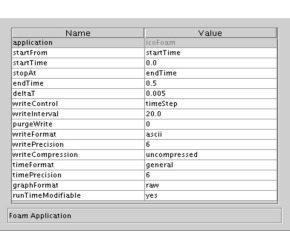
\includegraphics{fig-A-19}
 \caption{ディクショナリ画面の例:\OFdictionary{controlDict}}
 \label{fig:A.19}
\end{figure}


\index{Dictionaries@\OFemph{Dictionaries}!ディクショナリツリー}%
\index{ディクショナリツリー!Dictionaries@\OFemph{Dictionaries}}%
\OFemph{Dictionaries}のデータは編集可能です.ディクショナリは\autoref{fig:A.19}に示す
\OFdictionary{controlDict}や\autoref{sec:4.3},\autoref{sec:4.4},\autoref{sec:4.5}で
それぞれ示した\OFtool{fvSchemes}や\OFtool{fvSolution},
そして材料プロパティの元となるものを含んでいます.
ディクショナリは右欄にデータ入力箇所をもつ表形式の入力となっています.
入力箇所をクリックすることで値を直接編集でき,
また同じ方法により値が編集可能なサブディクショナリを開くこともできます.
例えば\autoref{fig:A.19}のapplicationClassのように
灰色で表示された入力箇所は編集できないので注意してください.
また入力箇所によってはSelection Editorから選択することもあり,
この場合には選択された入力欄は緑色にハイライトされます.


\subsection{データの保存}
\label{ssec:A.4.6}
ボタンバーからSave Case機能を選択すれば,
ケースへの変更を保存できます.
ディクショナリやフィールド,メッシュのデータが保存されます.


\subsection{ソルバの実行}
\label{ssec:A.4.7}
ソルバは二つの方法から選択して実行できます.
フォアグラウンドですぐに実行したい場合は,
ボタンバーからStart Calculation Now機能を選択します.
詳しい情報の表示なくOpenFOAMソルバはすぐに実行されます.

一方,ボタンバーからstart Calculation機能を選択することもできます.
これは\autoref{fig:A.20}に示すようにRun Applicationの画面を表示します.


\begin{figure}[ht]
 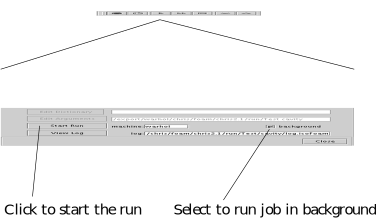
\includegraphics{fig-A-20}
 \caption{Start Calculation機能を使ったソルバの実行}
 \label{fig:A.20}
\end{figure}


Start Runボタンを押す前にバックグラウンドボタンをクリックすると,
バックグラウンドでケースは実行されます.
バックグラウンドで実行したケースの場合,
途中経過はログテキストボックスで指定されたログファイルに書かれ,
View Logボタンを押せば見ることができます.


\subsection{実行ユーティリティ}
\label{ssec:A.4.8}
OpenFOAMには多くのユーティリティが供給されており,
\autoref{fig:A.21}に示すようにケースサーバ画面で
ケース名アイコンをハイライトさせ,
右クリックでユーティリティを含むメニューの階層を開くことで実行できます.


\begin{figure}[ht]
 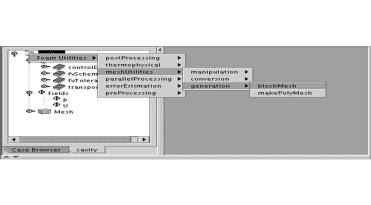
\includegraphics{fig-A-21}
 \caption{ユーティリティの実行}
 \label{fig:A.21}
\end{figure}


\autoref{fig:A.22}の例では
\OFtool{blockMesh}のユーティリティを選択すると,
もしそのユーティリティに関連のあるディクショナリがあれば編集画面が開きます.
必須のコマンドラインの変数は編集されているケースの
デフォルト値に設定されています.
ユーザは表から任意の変数を選択できます.


\begin{figure}[ht]
 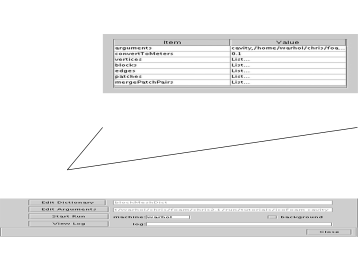
\includegraphics{fig-A-22}
 \caption{ユーティリティディクショナリの表示}
 \label{fig:A.22}
\end{figure}


\subsection{ケースサーバーの終了}
\label{ssec:A.4.9}
ケースサーバ画面を閉じて,ケースブラウザに戻るためには
Close Caseボタンをクリックしてください.



\section{\OFtool{FoamX}の設定}
\label{sec:A.5}
\OFtool{FoamX}ユーザ設定ファイルはユーザの
\OFpath{OpenFOAM-1.5/apps/FoamX}ディレクトリにあり,
ディレクトリの構造を保持しています.
そしてそのファイルはユーザの\OFpath{\$HOME}に
コピーされているかもしれません.
ユーザが設定可能なファイルは以下の通りです.
\begin{description}
 \item[\OFpath{FoamXClient.cfg}]
\index{FoamXClient.cfg@\OFpath{FoamXClient.cfg}!ファイル}%
\index{ファイル!FoamXClient.cfg@\OFpath{FoamXClient.cfg}}%
            では\OFtool{FoamX}のネットワークや外観を設定します.
            特に以下の設定が可能です.
            \begin{itemize}
             \item \texttt{org.omg.CORBA.ORBInitialHost=} や
                   \texttt{org.omg.CORBA.ORBInitialPort=} へ
                   入力することにより与えられるhost/portアドレスの設定.
             \item \texttt{FoamX.Browser=} を編集して
                   netscapeやmozilla,konqueror等のブラウザへの
                   入力を行ったり,URLが与えられている実行ファイルを
                   編集することによるデフォルトブラウザの設定.
             \item \texttt{FoamX.Editor=} に関連のある入力を
                   コメントアウト (\verb|#|) し,internalやnedit,
                   xemacs等からその編集を削除することによる
                   デフォルトエディタの設定.
            \end{itemize}
 \item[\OFpath{FoamX.cfg}]
\index{FoamX.cfg@\OFpath{FoamX.cfg}!ファイル}%
\index{ファイル!FoamX.cfg@\OFpath{FoamX.cfg}}%
            では編集可能なprocessControlを設定します.
            特に,リモート・シェルかセキュア・シェルの
            どちらを実行しているかによって
            rshまたはsshにremoteShellを設定します.
            このファイルでは接続の時間切れやコマンドの再試行に関する
            時間の設定もでき,問題が発生したときのコマンドを
            増やすこともできます.
\end{description}
\OFtool{FoamX}編集に関する環境変数は\OFpath{\$FOAMX\_}で始まり,
\autoref{tbl:A.3}に記載してあります.


\begin{table}[ht]
 %#! platex UserGuideJa
\begin{tabularx}{\textwidth}{lX}
 環境変数 & 説明とオプション \\
 \hline
\index{FOAMX PATH@\OFenv{FOAMX\_PATH}!かんきょうへんすう@環境変数}%
\index{かんきょうへんすう@環境変数!FOAMX PATH@\OFenv{FOAMX\_PATH}}%
 \OFenv{\$FOAMX\_PATH} &
     \OFtool{FoamX}インストールへのパス,\OFpath{\$FOAM\_UTIL/FoamX} \\
\index{FOAMX SYSTEM CONFIG@\OFenv{FOAMX\_SYSTEM\_CONFIG}!かんきょうへんすう@環境変数}%
\index{かんきょうへんすう@環境変数!FOAMX SYSTEM CONFIG@\OFenv{FOAMX\_SYSTEM\_CONFIG}}%
 \OFenv{\$FOAMX\_SYSTEM\_CONFIG} &
     \OFtool{FoamX}システム構成ファイルへのパス,\hfil\break
     \OFpath{\$FOAMX\_PATH/config} \\
\index{FOAMX USER CONFIG@\OFenv{FOAMX\_USER\_CONFIG}!かんきょうへんすう@環境変数}%
\index{かんきょうへんすう@環境変数!FOAMX USER CONFIG@\OFenv{FOAMX\_USER\_CONFIG}}%
 \OFenv{\$FOAMX\_USER\_CONFIG} &
     \OFtool{FoamX}ユーザ構成ファイルへのパス,\hfil\break
     \OFpath{\$HOME/\$FOAM\_DOT\_DIR/apps/FoamX} \\
 \hline
\end{tabularx}

 \caption{\OFtool{FoamX}の環境変数}
 \label{tbl:A.3}
\end{table}


\subsection{JAVA}
\label{ssec:A.5.1}
\OFtool{FoamX}ケースブラウザは必ず必要なバージョンというわけでは
ないかもしれませんが標準でインストールされているJAVA~1.5を使います.
そのためOpenFOAMに付属しており,
\index{JAVA HOME@\OFenv{JAVA\_HOME}!かんきょうへんすう@環境変数}%
\index{かんきょうへんすう@環境変数!JAVA HOME@\OFenv{JAVA\_HOME}}%
\OFenv{\$JAVA\_HOME}の環境変数はJAVAの最上位ディレクトリの
\OFpath{\$WM\_PROJECT\_DIR/.bashrc} (もしくは\OFpath{.cshrc}) における
デフォルトで決められています.
システム管理者は適宜\OFpath{\$JAVA\_HOME}の設定を行うことで,
代わりの場所にJAVA~1.5をインストールしても構いません.


\subsection{ケースファイルへのパス}
\label{ssec:A.5.2}
\OFtool{FoamX}は\OFpath{.OpenFOAM-1.5/controlDict}ファイルへの
\OFkeyword{caseRoots}の入力からユーザのケース・ファイルへのパスを見つけます.
デフォルトでは以下のように設定されています.
\begin{OFfile}
\begin{verbatim}
caseRoots
(
    "."
    "$FOAM_RUN/tutorials/icoFoam"
    "$FOAM_RUN/tutorials/turbFoam"
    ...
);
\end{verbatim}
\end{OFfile}
デフォルトでは
\index{FOAM RUN@\OFenv{FOAM\_RUN}!かんきょうへんすう@環境変数}%
\index{かんきょうへんすう@環境変数!FOAM RUN@\OFenv{FOAM\_RUN}}%
\OFenv{\$FOAM\_RUN}は
\OFpath{\$HOME/OpenFOAM/\$\{USER\}-1.5/run}のディレクトリを示します.
これは,デフォルトでは,\OFpath{run}ディレクトリにコピーされた
チュートリアルのディレクトリの中にあるケースや,
\OFtool{FoamX}が起動されるディレクトリの中のケースを開くことができることを意味します.
もしそれらパスを設定したい場合は,
\OFpath{\$HOME/.OpenFOAM-1.5}ディレクトリの
\OFdictionary{controlDict}ファイルのローカルコピーの中で設定を行ってください.
